\section{Análisis de Sistemas Tolerantes a Fallas en General}\label{sec:requerimentos_sistema_tolerancia_fallas}

%\section{Requerimientos de un Sistema con Tolerancia a Fallas}\label{sec:requerimentos_sistema_tolerancia_fallas}

% Primero se dan características de sistemas con redundancias de tiempo de tiempo real. De esto hay mucho en el libro de Kopetz y en su paper The Time Triggered Architecture. También en los papers que tengo impresos.

% Luego se menciona que esas características se hacen presente en varios de los trabajos de UAVs presentados en la sección anterior. Luego, explico los requerimientos como ya los tengo acá escritos.

% Volver a escribir la introducción a la sección
A partir de los distintos casos presentados, en esta sección se busca relevar cuáles son las características comunes en sistemas con tolerancia a fallas. Se analizan las distintas alternativas y luego se mencionan los criterios tenidos en cuenta para el desarrollo de la computadora de vuelo. En este trabajo no se define a priori cuál es la arquitectura del sistema en cuanto al uso de redundancias, por lo que la computadora de vuelo debe tener cierta diversidad en cuanto a sus capacidades.

\subsection{Características de Sistemas Tolerantes a Fallas}

El objetivo del diseño tolerante a fallas consiste en mejorar la confianza (\textit{Dependability}) del sistema, apuntando a que este pueda seguir ejecutando su función de manera correcta a pesar de la presencia de una cierta cantidad de fallas \cite{nelson1990fault}. De esta última expresión se puede tomar una definición de lo que es un sistema tolerante a fallas.

\begin{mydef}
    \textbf{Sistema Tolerante a Fallas:} es aquel donde una falla no implica necesariamente un fracaso en el funcionamiento. Un sistema tolerante a fallas no es aquel donde no ocurren fallas, sino que más bien, se acepta que las fallas pueden ocurrir en el sistema, pero lo que se pretende es que el sistema pueda cumplir con su función de igual manera.
\end{mydef}

De manera de introducir la nomenclatura que se encuentra en la bibliografía \cite{nelson1990fault}, se definen los siguientes términos:

\begin{itemize}
    \item Falla (\textit{Fault}): es alguna condición anómala, no esperada.
    \item Error: ocurre cuando una falla se manifiesta y produce un comportamiento fuera de lo esperado en alguna parte del sistema.
    \item Fracaso (\textit{Failure}): quiere decir que el sistema no puede cumplir con su función de manera adecuada.
\end{itemize}

Una de las formas de cuantificar la confianza es a través de la fiabilidad del sistema (\textit{Reliability}). Esta se expresa en la ecuación \eqref{eq:Reliability}, y se define como la probabilidad de que el sistema pueda cumplir su función de manera correcta en un intervalo de tiempo $[t_0;t]$, dado que en el instante inicial $t_0$ el sistema podía hacerlo.

\begin{equation}
    R(t) = \mathtt{P}\left( \text{funcionamiento correcto en $t$} | \text{funcionamiento correcto en $t_0$} \right)
    \label{eq:Reliability}
\end{equation}

Dado que en el intervalo $[t_0;t]$ puede o no ocurrir una falla, la probabilidad de que el sistema pueda cumplir su función en $t$ puede expresarse como en la ecuación \eqref{eq:Reliability_2}. Si no ocurre ninguna falla, luego el sistema podrá seguir cumpliendo su función en $t$. Además, si llegase a ocurrir una falla, pero el sistema tiene la capacidad de tolerarla, luego el sistema de igual manera podrá seguir cumpliendo su función en el instante $t$.

\begin{equation}
    \begin{aligned}
        R(t) &= \mathtt{P}\left( \text{no ocurrio una falla en $[t_0;t]$} \right)\\ &+ \mathtt{P}\left( \text{funcionamiento correcto en $t$}|\text{ocurrió una falla en $[t_0;t]$} \right) \ \mathtt{P}\left( \text{ocurrió una falla en $[t_0;t]$} \right)
    \end{aligned}
    \label{eq:Reliability_2}
\end{equation}

En el caso en el que se tuviera un sistema que no comprende ningún mecanismo de tolerancia a fallas, luego la fiabilidad sería exactamente igual a la probabilidad de que no ocurra una falla, ya que la ocurrencia de una falla causaría un funcionamiento incorrecto. Esto no necesariamente representa un problema. Si el sistema en cuestión es tal que puede demostrarse que la probabilidad de que no ocurra una falla es lo suficientemente alta, luego no se requeriría el uso de técnicas de tolerancia a fallas.

En un sistema donde no hay tolerancia a fallas, la fiabilidad quedaría definida como en la ecuación \eqref{eq:Reliability_3} y la única manera de mejorarla sería incrementando la probabilidad de que no ocurra ninguna falla en el intervalo $[t_0;t]$.

\begin{equation}
    R(t) = \mathtt{P}\left( \text{no ocurrio una falla en $[t_0;t]$} \right)
    \label{eq:Reliability_3}
\end{equation}

La manera de hacer esto puede ser por ejemplo, utilizando componentes o módulos de muy buena calidad, lo suficientemente confiables como para cumplir con los requerimientos de fiabilidad \cite{nelson1990fault}. Sin embargo, esto puede ser muy costoso, pensando en que un sistema puede tener una enorme cantidad de posibles fallas. No solo eso, sino que esto dificulta la etapa de diseño de un sistema, ya que cualquier error de diseño que no se haya tenido en cuenta puede llegar a causar una falla y por ende un fracaso del sistema. Por el contrario, la tolerancia a fallas plantea permitir que las fallas existan, pero aplicando técnicas para tolerarlas.

Volviendo a la ecuación \eqref{eq:Reliability_2}, la probabilidad de que el sistema funcione correctamente a pesar de la falla, está pesada por la probabilidad de ocurrencia de dicha falla. A partir de esto se desprende que aplicar técnicas de tolerancia a fallas para cada una de las posibles fallas puede resultar exhaustivo, principalmente porque deberían conocerse todas las fallas posibles, además de ser algo costoso. Lo que se propone es considerar solo aquellas fallas cuya criticidad es alta.

A modo de ejemplo, una \textbf{falla en un sensor de la computadora de vuelo puede generar una lectura incorrecta}. En consecuencia, esto decantará en un \textbf{error, es decir, en un cálculo de la ley de control incorrecto}. Finalmente, este error puede llevar al \textbf{fracaso de la misión, por ejemplo si el vehículo no es capaz de seguir una trayectoria dada en tiempo y forma}. Esto da a entender que una falla en un sensor es crítica y que por ende requiere la aplicación de técnicas de tolerancia a fallas.

Aquí se habla de falla en un sensor como algo general. Un sensor podría fallar de muchas maneras y debido a muchas razones. Por ejemplo, puede dejar de funcionar por un defecto propio del componente, puede entregar lecturas erróneas debido a interferencias electromagnéticas, por efectos de la temperatura, falta de calibración, etc. Cada uno de estos requeriría la aplicación de un mecanismo tolerante a fallas.

\subsection{Uso de Redundancias}

La principal técnica de tolerancia a fallas es el uso de redundancias \cite{nelson1990fault}\cite{prasad1989fault}\cite{lala1994architectural}\cite{kopetz2003time}. Esto quiere decir, que se replica el hardware en el sistema y cada réplica realiza la misma tarea en paralelo. De esta forma, si una de las réplicas presenta una falla (arbitraria por ejemplo), esta puede detectarse a partir de la comparación con las demás réplicas, o incluso pasar desapercibida. Utilizando la nomenclatura definida en la sección \ref{subsec:introduccion_al_analisis_de_tolerancia_a_fallas}, que una falla pase desapercibida quiere decir que no se manifiesta como un error, sino que esta es contenida. A continuación se presentan algunas arquitecturas redundantes para la tolerancia a fallas.

\subsubsection*{Redundancia Doble}

Una arquitectura simple es la redundancia doble. En este tipo de sistemas, dos nodos de un sistema funcionan en paralelo y comparan sus resultados. La comparación permite detectar si los resultados difieren entre sí, lo que se traduce en que ocurrió un error.

\begin{figure}[H]
    \centering
    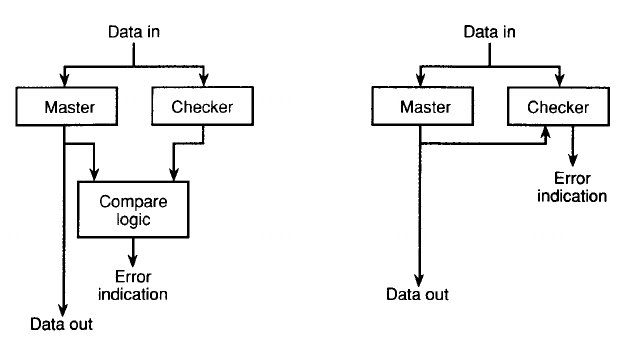
\includegraphics[width=0.6\textwidth]{img/3_4_lockstep_architecture.png}
    \caption{En la figura de la izquierda, dos sistemas ejecutan las mismas operaciones, mientras que otro sistema externo se encarga de comparar las salidas de ambos para detectar errores. En la figura de la derecha, el bloque comparador se encuentra integrado en el sistema \textit{checker}. La imagen fue extraida de \cite{nelson1990fault}.}
    \label{fig:3_4_lockstep_architecture}
\end{figure}

Este tipo de arquitectura permite detectar si ocurrió un error, pero no permite identificar de qué nodo proviene el error. En la figura \ref{fig:3_4_lockstep_architecture} se muestran dos configuraciones. La configuración de la derecha puede ser implementada a través de dos CPUs totalmente independientes (a veces denominada \textit{Loosely-Synchronized Dual Processor Architecture}) o a través del uso de un procesador de dos núcleos, donde uno sería el \textit{Master} y otro el \textit{checker}\cite{baleani2003fault}. En esta última, ambos se encuentran sincronizados por estar en el mismo chip y compartir fuente de clock. En la figura \ref{fig:3_4_lockstep_architecture_2} se muestra un esquema de ambos casos.

\begin{figure}[H]
    \centering
    \begin{subfigure}[b]{0.49\textwidth}
        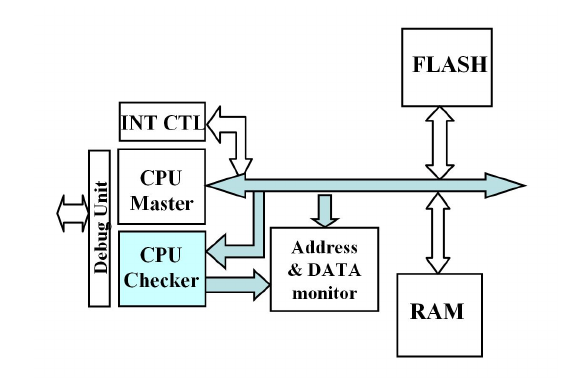
\includegraphics[width=\textwidth]{3_4_lockstep_dual_core.png}
        \caption{Lockstep dual processor architecture.}
        \label{fig:3_4_lockstep_dual_core}
    \end{subfigure}
    \begin{subfigure}[b]{0.49\textwidth}
        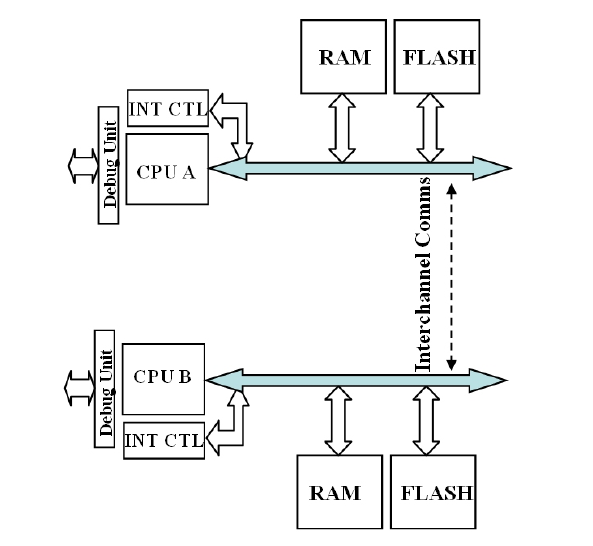
\includegraphics[width=\textwidth]{3_4_loosely_synchronized_dual_processor_architecture.png}
        \caption{Loosely synchronized dual processor architecture.}
        \label{fig:3_4_loosely_synchronized_dual_processor_architecture}
    \end{subfigure}
    \caption{Se muestran dos casos para un sistema con redundancia doble. La imagen fue extraida de \cite{baleani2003fault}.}
    \label{fig:3_4_lockstep_architecture_2}
\end{figure}

Debido a que no se puede saber cuál de las dos CPUs cometió el error, esta arquitectura plantea que en el caso en el que la comparación entre ambas CPUs genere una discrepancia en los resultados, cada una de ellas deben ejecutar un algoritmo interno, para detectar si ellas fueron las que cometieron el error o no. En \cite{zhang2015dual} y en \cite{SolanoPerez2019} se pueden encontrar proyectos de redundancia doble para UAVs.

\subsubsection*{Redundancia Triple}

Esta arquitectura puede encontrarse en la literatura con el nombre \textit{Triple Modular Redundant (TMR) Architecture} \cite{baleani2003fault}\cite{nelson1990fault}\cite{prasad1989fault}\cite{lyons1962use}. Esta arquitectura consiste en utilizar tres computadoras en paralelo, las cuales computan los mismos resultados. Luego, se comparan los resultados. Se asume que solamente 1 de las 3 presentará una falla a la vez. En dicho caso, los resultados de dos computadoras serán iguales y la de la tercera será distinto, por lo que solamente se descarta el resultado erróneo. En la figura \ref{fig:3_5_TMR} se muestra un diagrama con la arquitectura TMR. Una diferencia de esta arquitectura respecto de la doble redundancia, es el hecho de que puede detectarse cuál de las computadoras falló y además, no es necesario que todas las computadoras ejecuten una rutina para verificar si cometieron el error o no. Esto resulta especialmente útil en sistemas de tiempo real, donde no puede detenerse el sistema para realizar una verificación interna. Esto se denomina \textit{Fault Masking}.

\begin{figure}[H]
    \centering
    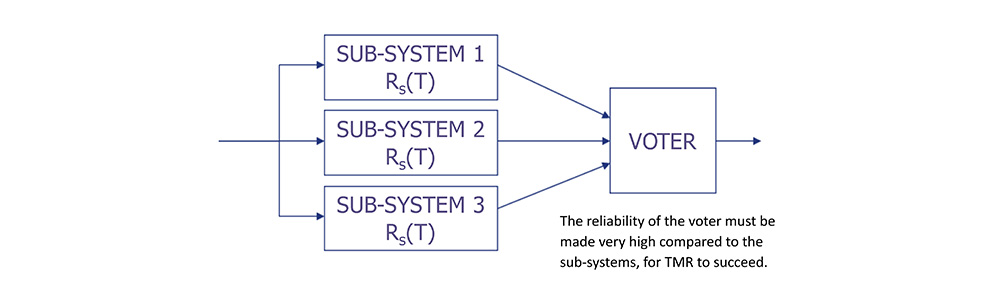
\includegraphics[width=0.8\textwidth]{3_5_TMR.png}
    \caption{Arquitectura TMR. La imagen fue extraida de \cite{TMRwebPage}.}
    \label{fig:3_5_TMR}
\end{figure}

Como indica el texto de la imagen, una cuestión clave de esta arquitectura es el bloque denominado \textit{VOTER}. Debido a que este bloque es el que determina cuál es el resultado correcto, se requiere que la fiabilidad, $R(t)$, de este sea mucho mayor que la de cada computadora de vuelo. Esto se logra a través del uso de hardware más robusto, lo que resulta en que el bloque \textit{VOTER} sea más costos que cada computadora de vuelo. Por ejemplo, cada computadora de vuelo puede comprender un microcontrolador COTS, mientras que el bloque voter puede estar implementado con un ASIC específico para esa aplicación \cite{hiergeist2017internal}. Si bien este bloque tiene una fiabilidad mucho mayor, siempre existe la probabilidad de que ocurra un error en este. En cuyo caso, el error puede decantar en un fracaso, por ejemplo si el \textit{VOTER} elige como resultado correcto, aquel que realmente no lo era.

\begin{mydef}
    \textbf{Single-Point Failure}: si la arquitectura del sistema es tal que una parte del sistema X fracasa en cumplir su trabajo dentro del sistema, luego el sistema completo fracasará en cumplir su función. En dicho caso, X es un punto único de falla.
\end{mydef}

Una forma de combatir esto es replicar los bloques que realizan la votación \cite{nelson1990fault}\cite{lyons1962use}. De esta manera, también pueden enmascararse errores de los bloques que realizan la votación. La arquitectura sería como la que se muestra en la figura \ref{fig:3_3_2_consenso_1}.

\begin{figure}[H]
    \centering
    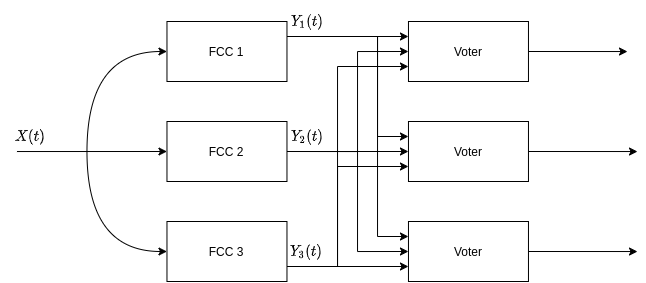
\includegraphics[width=0.7\textwidth]{img/3_4_2_consenso_1.png}
    \caption{Arquitectura TMR con redundancia en los elementos votantes.}
    \label{fig:3_3_2_consenso_1}
\end{figure}

Los tres elementos \textit{Voter} reciben las mismas entradas y en el caso de que ninguno de los \textit{voters} cometa un error, dado que las entradas de los \textit{Voters} son exactamente iguales, luego los tres decidirán por el mismo resultado como el valor correcto.

Esta arquitectura es más compleja que las anteriores, ya que requiere una gran cantidad de nodos, 3 FCCs + 3 bloques votantes, dando un total de 6. Además, pensando en que se argumentó que los votantes generalmente son más confiables que las FCCs, la triplicación del bloque \textit{Voter} encarece mucho al UAV.

%Otra cuestión que aparece en esta arquitectura, es que si bien los votantes generan cada uno un valor de salida, al fin y al cabo será uno solo el valor a utilizar. En la figura \ref{fig:3_3_2_consenso_1}, cada voter tiene su propia salida, pero en algún punto se deberá decidir cuál de las tres salidas es la que se va a utilizar como correcta. Por ejemplo, si el valor de salida es la señal de actuación de un motor, luego los tres resultados del voter deberan enviarse a algún modulo encargado de controlar dicho motor.

Como medida para evitar esto último, los bloques votantes pueden integrarse dentro de cada una de las FCC. Esto quiere decir, que en lugar de tener 3 bloques votantes, las mismas FCC sean las encargadas de realizar la votación. En el artículo \cite{hiergeist2017internal} se propone que los microcontroladores automotivos ofrecen las interfaces necesarias para implementar una red redundante para tolerar fallas. En el artículo \cite{hiergeist2018implementation}, los mismos autores presentan resultados para una arquitectura con redundancia cuádruple, donde los mismos microcontroladores de cada FCC son los encargados de realizar la votación. Para el caso de una arquitectura de redundancia triple, puede diagramarse como en la figura \ref{fig:3_5_TMR_2}.

\begin{figure}[H]
    \centering
    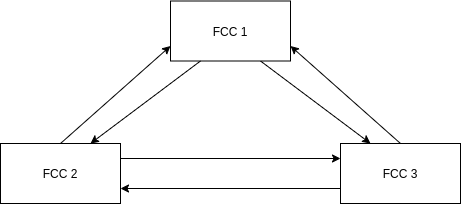
\includegraphics[width=0.5\textwidth]{img/3_5_TMR_2.png}
    \caption{Arquitectura de redundancia trple, donde los bloques votantes son las mismas FCCs. Los votantes se encuentran integrados dentro de cada FCC.}
    \label{fig:3_5_TMR_2}
\end{figure}

\subsection{Requerimientos Comunes en Sistemas con Redundancias}

Todos los trabajos y ejemplos presentados en la sección anterior comparten la característica de implementar la tolerancia a fallas utilizando varias copias del mismo elemento de hardware. Estas copias trabajan en paralelo y se comparan los resultados obtenidos por cada una de ellas. Las fallas se detectan cuando ocurre una diferencia en los resultados de las copias.\\

{\color{red} EXPLICAR Y JUSTIFICAR EL POR QUÉ DE LAS REDUNDANCIAS POR SOBRE EL USO DE COMPONENTES DE ALTÍSIMA CALIDAD, EN UN PÁRRAFO.}

A continuación, se describen algunas de las características detectadas.

\subsubsection{Sincronismo de los Nodos}
%\subsection{Sincronismo de los Nodos}

Prácticamente en todos los trabajos presentados se menciona que los nodos reundantes trabajan de manera sincronizada. Esta necesidad surge debido a que las comparaciones se realizan sobre variables que cambian en el tiempo y que tienen validez solamente durante un período de tiempo. Esto es algo característico de sistemas de tiempo real, ya que un dato de un sensor $X(t)$ solamente tendrá validez durante un breve período de tiempo. 
%En las arquitecturas antes presentadas, se menciona que se realiza una comparación de los resultados calculados por cada nodo, para detectar/enmascarar errores. Para que el funcionamiento de esta comparación sea adecuado, los nodos deben estar sincronizados. Esto es un requerimiento para sistemas de tiempo real, como el caso de la computadora de vuelo de un UAV.
En la figura \ref{fig:3_4_1_sincronizacion} se muestra un ejemplo. En el instante $t$, se presenta una nueva medición de un sensor a las tres computadoras de vuelo. Al comienzo de la misión, todas ellas estarán sincronizadas y generarán un resultado del cálculo de la ley de control que corresponde al mismo intervalo de tiempo. Luego, se realiza la votación para elegir el valor correcto. La figura \ref{fig:3_4_1_sincronizacion_2}, muestra lo que sucede al cabo de un período de tiempo. Se presenta una nueva medición de un sensor en el instante $t$. Debido a la desincronización, es posible que las computadoras de vuelo no presenten sus resultados al árbitro a tiempo, por lo que este asumirá que una de las FCCs no presentó ninguna respuesta. Este caso suele estar contemplado dentro de las posibilidades y correpsonde al caso en el que una computadora de vuelo presentó un error y debido a ello no respondió con ningún valor (por ejemplo, se reinició su procesador debido a un \textit{watchdog}). En esos casos el árbitro simplemente asume algún valor por defecto.

\begin{figure}[H]
    \centering
    \begin{subfigure}[b]{0.49\textwidth}
        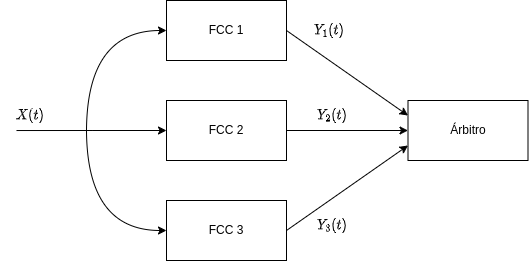
\includegraphics[width=\textwidth]{img/3_4_1_sincronizacion_1.png}
        \caption{Computadoras de vuelo al inicio de la misión.}
        \label{fig:3_4_1_sincronizacion_1}
    \end{subfigure}
    \begin{subfigure}[b]{0.49\textwidth}
        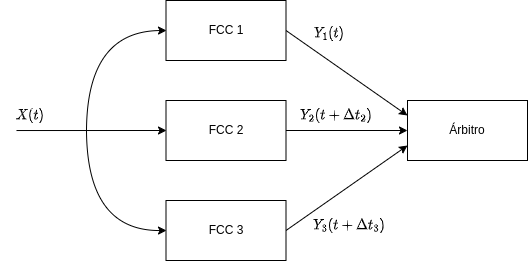
\includegraphics[width=\textwidth]{img/3_4_1_sincronizacion_2.png}
        \caption{Al cabo de un período de tiempo, se desincronizarán.}
        \label{fig:3_4_1_sincronizacion_2}
    \end{subfigure}
    \caption{A medida que transcurra el tiempo, la desincronización entre FCCs impactará en el sistema redundante.}
    \label{fig:3_4_1_sincronizacion}
\end{figure}

Otra situación que puede presentarse, es que los resultados propuestos por las computadoras de vuelo $Y_1$, $Y_2$ e $Y_3$ correspondan a intervalos de tiempo distintos. Este caso es todavía peor que el anterior, ya que no se encuentra contemplado y el árbitro simplemente realizará la votación asumiendo que el dato es válido.

\begin{figure}[H]
    \centering
    \begin{subfigure}[b]{0.49\textwidth}
        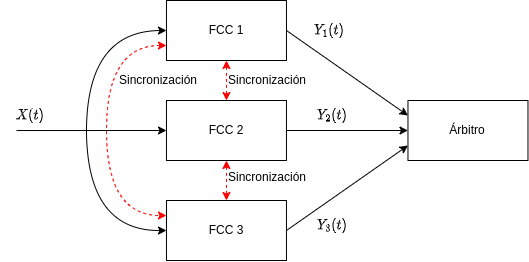
\includegraphics[width=\textwidth]{img/3_4_1_sincronizacion_3.png}
        \caption{Las mismas computadoras de vuelo se encargan de la sincronización.}
        \label{fig:3_4_1_sincronizacion_3}
    \end{subfigure}
    \begin{subfigure}[b]{0.49\textwidth}
        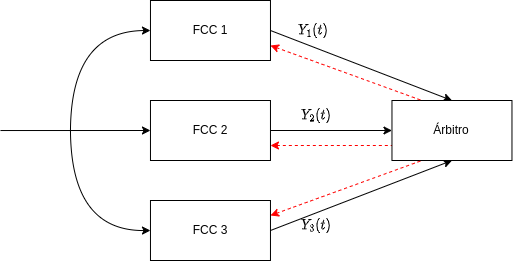
\includegraphics[width=\textwidth]{img/3_4_1_sincronizacion_4.png}
        \caption{En este caso, la sincronización es administrada por el árbitro.}
        \label{fig:3_4_1_sincronizacion_4}
    \end{subfigure}
    \caption{La sincronización entre nodos es necesaria para un correcto funcionamiento de las redundancias.}
\end{figure}

Se concluye que es mandatorio utilizar alguna técnica de sincronización entre los nodos. Como detalle de la figura \ref{fig:3_4_1_sincronizacion_3}, se muestra que la sincronización entre nodos presupone otro canal de comuniación más. Otra forma podría ser relegar la tarea de la sincronización al árbitro, aunque esto nuevamente presenta un punto singular de falla. Como se demostró en esta sección, el sincronismo es un aspecto crítico en el sistema redundante, por lo que se prefiere evitar esto último. Aunque de todas formas quisiera relegarse la sincronización al árbitro, este no solo recibirá mensajes de cada una de las FCCs, sino que además les enviará mensajes. Esto se muestra en la figura \ref{fig:3_4_1_sincronizacion_4}. Puede ocurrir una situación en la que el árbitro entregue valores distintos a cada una de las FCCs, evitando que estas se sincronicen.

\subsubsection{Consenso}\label{sec:consenso}
%\subsection{Consenso}\label{sec:consenso}

Como se mostró en la figura \ref{fig:3_4_1_sincronizacion_3}, las computadoras de vuelo pueden comunicarse entre ellas para lograr una sincronización, por ejemplo compartiendo a sus pares un valor asociado a su propio clock interno. Cada FCC propone un valor distinto y estas buscarán ponerse de acuerdo en un valor único. Para que cada una de ellas llegue a la misma conclusión acerca del valor de clock correcto, si todas ellas ejecutan el mismo algoritmo y poseen los mismos valores de entrada, luego llegarán a la misma conclusión. En la figura \ref{fig:3_4_2_consenso_4} se muestra un caso en el que una de las computadoras de vuelo comparte valores de clock distintos a sus pares.

\begin{figure}[H]
    \centering
    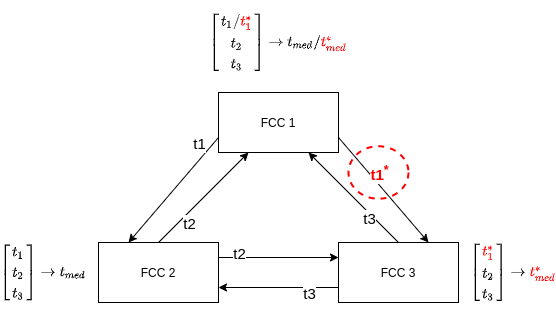
\includegraphics[width=0.6\textwidth]{img/3_4_2_consenso_4.png}
    \caption{La FCC1 entrega un valor distinto de timing a las demás FCCs}.
    \label{fig:3_4_2_consenso_4}
\end{figure}

En este escenario, la FCC1 entrega dos valores distintos de su clock a las demás FCCs. Cada una de ellas luego realiza un promedio para llegar a un único valor. Lo que se observa es que las FCC2 y FCC3 calcularán un valor promedio distinto, es decir, no se sincronizarán.
Una posible solución podría ser que las FCCs hagan un nuevo intercambio, con los valores promedio calculados y realicen una votación interna. Esto se muestra en la figura \ref{fig:3_4_2_consenso_5}.

\begin{figure}[H]
    \centering
    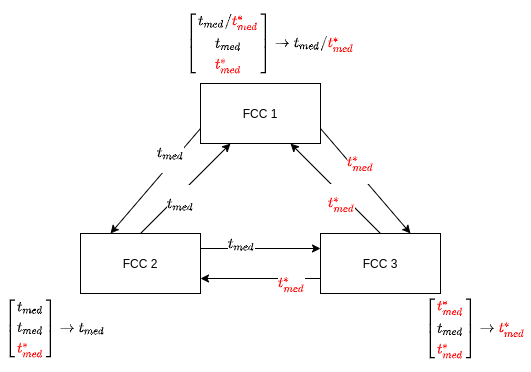
\includegraphics[width=0.6\textwidth]{img/3_4_2_consenso_5.png}
    \caption{Luego de calcular los promedios, las FCCs intercambian sus resultados. Nuevamente, la FCC1 comete una falla en el envío del dato.}
    \label{fig:3_4_2_consenso_5}
\end{figure}

Esta última situación, donde la FCC1 nuevamente comparte dos valores distintos a las demás, puede llevar a que las computadoras de vuelo no se sincronicen, algo que como ya se mencionó, es crítico para la correcta ejecución del algoritmo de tolerancia a fallas. Podría argumentarse que es demasiado pesimista pensar que la FCC1 puede producir la misma falla 2 veces de manera consecutiva, ya que existe una baja probabilidad de que ello suceda. Sin embargo, la situación planteada en esta sección puede tratarse como un tipo de falla de hardware que se manifiesta como comportamientos arbitrarios. Que exista una sincronización entre nodos redundantes implica que estos llegan a un consenso del paso del tiempo y el ritmo al que deben ejecutar sus tareas asignadas. Este consenso resulta crítico para que el sistema pueda detectar fallas correctamente.\\

Algunos de los trabajos presentados anteriormente además realizan el algoritmo de votación sin la inclusión de un árbitro. Este caso es idéntico al de la figura \ref{fig:3_4_2_consenso_4}, es decir que el mismo problema del consenso también está presente para las votaciones acerca de resultados de cálculo de ley de control.\\

El modelo de falla que se está considerando representa un comportamiento anómalo arbitrario, es decir, que a priori no se asume nada acerca de la falla. A este tipo de comportamiento se lo denomina falla bizantina o \textit{Byzantine Fault} en inglés y básicamente consiste en asumir que el elemento que manifiesta la falla presenta un comportamiento arbitrario. Por ejemplo, un sensor puede dejar de funcionar repentinamente y no dar más respuesta, puede dejar de enviar respuesta por un período de tiempo y luego volver a funcionar, podría también enviar datos a un microcontrolador pero que esos datos sean incoherentes, etc. El modelo de falla bizantina no asume modos de falla, sino que el comportamiento es arbitrario \cite{roth2021not}\cite{hiergeist2017internal}\cite{lala1994architectural}. El nombre proviene de un problema denominado \textit{The Byzantine Generals Problem}, formalizado en \cite{lamport2019byzantine}. Otros trabajos que tratan el mismo problema son \cite{pease1980reaching} y \cite{wensley1978sift}. Este último, presenta el diseño de una computadora de vuelo tolerante a fallas que utiliza los resultados del \textit{Byzantine Generals Problem} para realizar distintas tareas de redundancia.\\

%Una forma de alivianar esta tarea es la de considerar un modelo de falla de hardware más conservador, donde se asume que una falla de hardware consiste en que esta presente un comportamiento anómalo arbitrario, es decir, de cualquier tipo. A este tipo de comportamiento se lo denomina falla bizantina o \textit{Byzantine Fault} en inglés y básicamente consiste en asumir que el elemento que manifiesta la falla presenta un comportamiento arbitrario. Por ejemplo, un sensor puede dejar de funcionar repentinamente y no dar más respuesta, puede dejar de enviar respuesta por un período de tiempo y luego volver a funcionar, podría también enviar datos a un microcontrolador pero que esos datos sean incoherentes, etc. El modelo de falla bizantina no asume modos de falla, sino que el comportamiento es arbitrario \cite{roth2021not}\cite{hiergeist2017internal}\cite{lala1994architectural}. Se define un sistema tolerante a este tipo de fallas.

Se plantea una situación como la de la figura \ref{fig:3_4_2_consenso_4}, pero en este caso se utilizan 4 computadoras de vuelo en lugar de 3. En este caso, las computadoras de vuelo deben sincronizarse. Para lograrlo, ellas comparten un valor de timestamp, que pueden utilizar para ajustar sus clocks. En la figura \ref{fig:Byzantine_Generals_Problem_5} se muestra un escenario en el que una de las computadoras de vuelo presenta una falla tal que le informa un valor distinto a cada una de sus pares.

\begin{figure}[H]
    \centering
    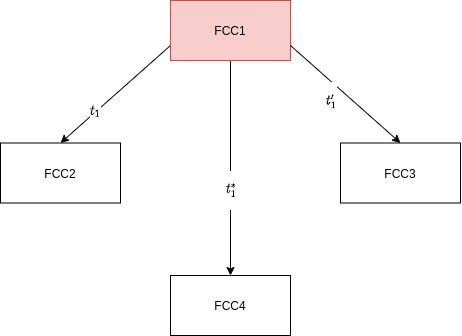
\includegraphics[width=0.5\textwidth]{img/Byzantine_Generals_Problem_5.png}
    \caption{Debido a una falla, la computadora de vuelo 1 le entrega valores distintos de timestamp a las demás.}
    \label{fig:Byzantine_Generals_Problem_5}
\end{figure}

\begin{figure}[H]
    \centering
    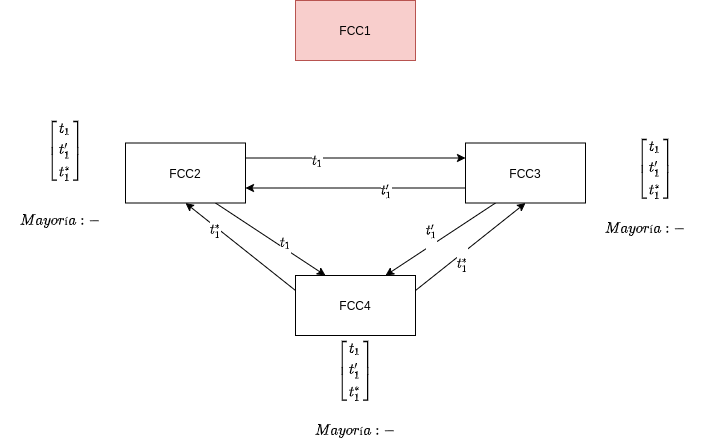
\includegraphics[width=0.7\textwidth]{img/Byzantine_Generals_Problem_6.png}
    \caption{Las FCC2, 3 y 4 comparten entre sí lo que les dijo la FCC1 a cada una y llegan a la conclusión de que la información es inconsistente.}
    \label{fig:Byzantine_Generals_Problem_6}
\end{figure}

A través de un segundo intercambio, las FCC 2, 3 y 4 llegan a la conclusión de que el timestamp de la FCC1 no es claro. En este caso, descartan el valor. Luego de hacer todos los intercambios de timestamp, las FCCs podrán aplicar internamente la sincronización, por ejemplo, calculando un promedio de todos los timestamp. \textbf{Dado que todas las FCCs tendrán la misma información de timestamp entregado por las demás FCCs, luego todas llegarán al mismo promedio y se sincronizarán}.\\

Un aspecto interesante es el hecho de que en el paper original, se hace una analogía entre un nodo redundante con fallas y un nodo traidor, es decir, que busca corromper el consenso de los demás nodos. Esto lo que quiere decir es que las fallas presentadas por las computadoras de vuelo pueden ser justamente de cualquier característica, incluso al extremo de presentar un comportamiento malicioso, con el objetivo de perjudicar al sistema \cite{lala1994architectural}. Esto sienta las bases para la tolerancia a fallas de hardware arbitrarias.\\

La implementación del algoritmo tolerante a fallas arbitrarias resulta costoso. Para poder tolerar fallas provenientes de 1 FCC se requiere un total de 4 computadoras de vuelo. Además, debe haber una interconexión entre las 4 computadoras y ellas deben intercambiar información continuamente para poder detectar y enmascarar la falla. A todo esto se le debe sumar, la necesidad de la sincronización.\\

\subsection{Simplificación del Problema}

Una de las cuestiones que no se menciona en el problema original, es el caso en el que los nodos constituyen sistemas de tiempo real. Las computadoras de vuelo deben realizar tareas que requieren determinismo temporal, por ejemplo cálculo de la ley de control, estimación de la pose, etc... En el problema original, los nodos pueden enviar sus mensajes a sus pares en cualquier momento y en cualquier orden. Otro de los puntos que caracterizan al problema original, es el hecho de que la comunicación entre los nodos es 1 a 1. Debido a esto, los traidores pueden entregar información confusa a sus pares para tratar de romper el consenso. Esto es lo que vuelve complejo al problema \cite{lamport2019byzantine} y costosa a su solución \cite{roth2021not}. Si el sistema en cuestión presenta la características de ser de tiempo real e implementar una comunicación a través de un bus, en conjunto, luego el problema del consenso puede simplificarse mucho.\\

En sistemas de tiempo real para aplicaciones \textit{safety-critical}, es común encontrar sistemas distribuidos con comunicación a través de un bus. Esto se mencionó en la sección \ref{sec:estado_del_arte} tanto para el caso del avión como para varios de los ejemplos de UAVs presentados. Esto tambień ocurre por ejemplo en los automóviles, los nodos que se encuentran repartidos por todo el vehículo se comunican a través de redes como CAN\cite{specification1991bosch} o FlexRay\cite{nxpAN12233}. Todos los nodos de la red se encuentran conectados al mismo bus de comunicación, por lo que cuando un nodo envía un mensaje a través del bus, todos los demás nodos reciben el mismo mensaje.

\begin{figure}[H]
    \centering
    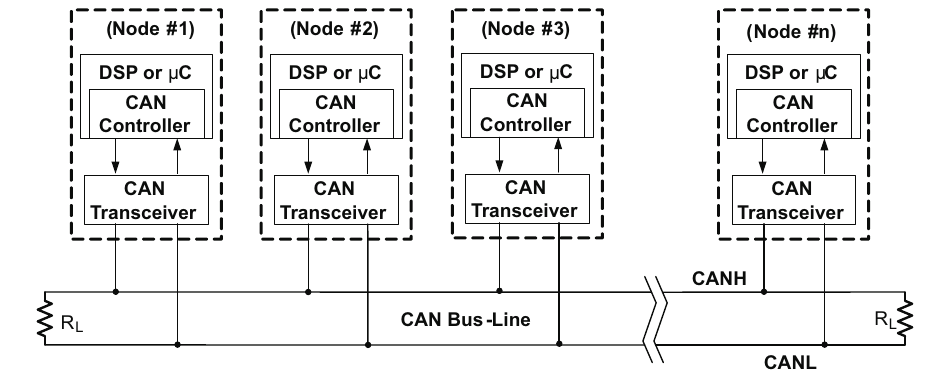
\includegraphics[width=\textwidth]{img/red_CAN.png}
    \caption{Todos los nodos se encuentran conectados al mismo bus de comunicaciones. En el caso del bus CAN, se compone de dos cables, CAN-H y CAN-L, terminados en sus extremos por resistencias de adaptación. La imagen se extrajo de \cite{texasSLOA101B}.}
    \label{fig:red_CAN}
\end{figure}

Esto presenta una diferencia respecto de lo planteado en \textit{The Byzantine Generals Problem}, ya que la existencia de un bus común a todos los nodos automáticamente elimina la posibilidad de que uno de los miembros de la red pueda enviar información diferente a sus pares. Puede compararse la figura \ref{fig:byzantine_bus_1} con la figura \ref{fig:Byzantine_Generals_Problem_5}.

\begin{figure}[H]
    \centering
    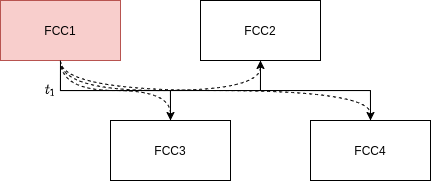
\includegraphics[width=0.6\textwidth]{img/byzantine_bus_1.png}
    \caption{En este caso, la conexión tipo bus no permite el envío de información diferente a los demás miembros. La FCC1 envía el valor $t_1$ y todos sus pares reciben el mismo valor.}
    \label{fig:byzantine_bus_1}    
\end{figure}

Como contrapartida, debido a que los nodos comparten canal de comunicación, estos deben tomar turnos para enviar la información a sus pares. De otra forma, habría una colisión en el bus y la información nunca llegaría a su destino. Sumado a esto, el bus se convierte en un punto singular de falla, ya que es posible que un problema en el bus deje a los nodos incomunicados.\\

%\subsubsection{Consenso}

Al igual que como se hizo en la sección \ref{sec:consenso}, se analiza el problema del consenso utilizando un bus. El ejemplo que se presentó anteriormente fue el necesario para lograr una sincronización entre las FCCs y se mostró que el enviar información distinta a cada computadora de vuelo puede romper el sincronismo muy fácilmente.\\

Como ya se mencionó, las FCCs deben tomar turnos para utilizar el medio físico. En las próximas secciones se explicará cómo se puede lograr esto, aquí se asume que las FCCs respetan sus turnos para utilizar el medio físico compartido. En la figura \ref{fig:byzantine_bus_2}, la FCC1 accede al medio y envía su valor de timestamp. Las demás FCCs reciben el mismo valor, por estar conectadas al mismo bus de comunicación. Luego, las FCC2 y 3 repiten esto mismo. En la figura \ref{fig:byzantine_bus_3} se muestra que todas tienen la misma información respecto de sus pares. Luego por ejemplo, si calculan un promedio, llegarán al mismo resultado y se sincronizarán correctamente.

\begin{figure}[H]
    \centering
    \begin{subfigure}[b]{0.34\textwidth}
        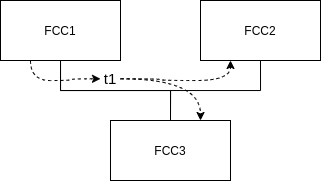
\includegraphics[width=\textwidth]{img/byzantine_bus_2.png}
        \caption{La FCC1 envía su \textit{timestamp} hacia las demás.}
        \label{fig:byzantine_bus_2}
    \end{subfigure}\hfill
    \begin{subfigure}[b]{0.49\textwidth}
        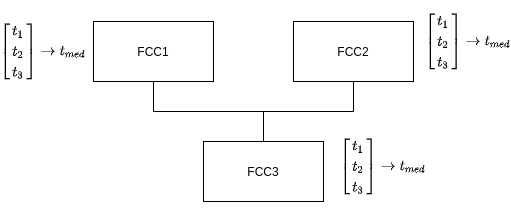
\includegraphics[width=\textwidth]{img/byzantine_bus_3.png}
        \caption{Luego de finalizar los intercambios, todas las FCCs llegan al mismo resultado de \textit{timestamp} para sincronizarse.}
        \label{fig:byzantine_bus_3}
    \end{subfigure}
    \caption{Debido a la existencia del bus, las FCCs no pueden mentir acerca de su \textit{timestamp}. Luego, todas llegan a un consenso de manera casi trivial.}
    \label{}
\end{figure}

A partir de este análisis, se puede ver que para el caso de un sistema de tiempo real con un único bus de comunicaciones, el problema del consenso es mucho más sencillo que lo que se muestra en \textit{The Byzantine Generals Problem}. De todas maneras, lo que se presenta aquí es un primer análisis, ya que se ha asumido que no hay colisiones en el bus y que los nodos se encuentran sincronizados. Se concluye que, para que la computadora de vuelo pueda implementar distintos mecanismos de tolerancia a fallas, esta debe contar con una interfaz que le permita la comunicación a través de un bus de comunicaciones.\\

\subsection{Uso de Componentes COTS}

\textbf{{\color{red} COMPLETAR}}

\subsection{Selección del Bus de Comunicaciones de la Computadora de Vuelo}

Como ya fue mencionado, la computadora de vuelo requiere de una interfaz para un bus de comunicaciones. A partir de lo presentado hasta aquí el único requerimiento es el método de acceso al medio, el cual debe ser controlado por el tiempo. Teniendo en cuenta que se trata de un trabajo realizado con componentes COTS, el hardware a utilizar debe ser de fácil acceso y con costos razonables. Para el desarrollo de este trabajo, se seleccionó el bus \textit{Controller Area Network} (CAN)\cite{specification1991bosch}. 

%En las secciones siguientes se explica un inconveniente, en cuanto a la selección del microcontrolador. 

El microcontrolador que se utiliza cuenta con un periférico que permite utilizar una interfaz con este bus. A continuación se presentan brevemente algunas características. Si bien el método de acceso al medio no es TDMA, existe una extensión del protocolo que justamente busca incorporar esta funcionalidad en otra capa superior.

\subsubsection{Descripción del Protocolo CAN}

El protocolo CAN fue desarrollado para ser usado en la industria automotriz, como bus de comunicación que conecta distintos módulos dentro de un automóvil. El objetivo de su desarrollo fue similiar al motivo por el cual se desarrolló el bus ARINC 629, reemplazar la gran cantidad de cables dentro del vehículo por un bus simple. El protocolo se corresponde con el modelo OSI y la especificación original define las capas física y de enlace, ISO 11898.\\

Cada nodo de un bus CAN se conecta a este a través de 2 cables, los cuales llevan la señal diferencial. Esto se muestra en la figura \ref{fig:conxeion_al_bus_CAN}. Todo el bus CAN se compone de 2 cables que llevan los mensajes a todos los nodos de la red. El hecho de que se trate de una señal diferencial hace que la comunicación sea robusta, reduciendo las emisiones electromagnéticas generadas por este. A su vez, es común que el bus sea cableado como un par trenzado, lo que atenúa señales de modo común, producto de cualquier acoplamiento. 

\begin{figure}[H]
    \centering
    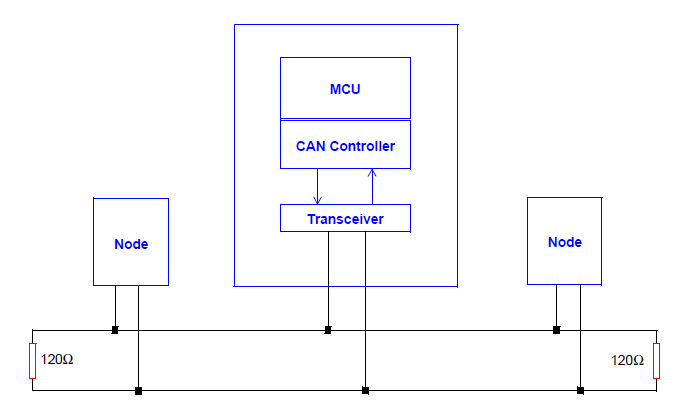
\includegraphics[width=0.5\textwidth]{img/conxeion_al_bus_CAN.png}
    \caption{La conexión de un nodo al bus es a través de 2 cables que llevan dos señales, CAN-H y CAN-L. La imagen se extrajo de \cite{AN228}.}
    \label{fig:conxeion_al_bus_CAN}    
\end{figure}

Existen muchas versiones del protocolo CAN, en este trabajo se utiliza la versión CAN High Speed. Esta define una velocidad máxima de transferencia de 1 Mbps, para un bus de hasta 40 m de longitud y 30 nodos conectados al mismo bus. Se recomienda que la conexión entre cada nodo y el bus no sea de más de 30 cm. El hecho de poder tener hasta 30 nodos expande las posibilidades de uso del bus, más allá de ser el medio principal de comunicación utilizado para el sistema redundante. Por ejemplo, distintos sensores o incluso actuadores como los motores del vehículo podrían conectarse al bus. {\color{red} Acá tendría que agregar alguna referencia a este uso del bus CAN}.\\

La impedancia característica del bus debe ser de $120 \ \Omega$. Es común agregar resistores de terminación en ambos extremos, para evitar reflexiones. En algunos casos pueden llegar a encontrarse aplicaciones donde los resistores de terminación se incluyen dentro de alguno de los nodos del bus. Esto no es recomendable, ya que si este se desconecta de forma accidental del bus, todas las comunicaciones entre los demás nodos se verán perjudicadas.\\

En la figura \ref{fig:conxeion_al_bus_CAN} se muestran 2 elementos que forman parte del nodo, el \textit{trasnciever} y el \textit{controller}. El primero de ellos forma parte de la capa física y es un circuito que convierte las señales diferenciales del bus en señales de modo común, que luego son transferidas al elemento \textit{controller}. Este componente sirve como interfaz física con el bus.\\

CAN es un protocolo donde no hay un nodo master, sino que todos pueden utilizar el medio para transmitir mensajes, mientras el bus no esté en uso. El método de acceso al medio que se utiliza es \textit{Carrer Sense Multiple Access with Collision Detection and Arbitration on Message Priority} (CSMA/CD+AMP). Antes de transmitir un mensaje, el nodo sensa el medio físico y en caso de que esté libre, intenta utilizarlo. En caso de que más de un nodo quiera enviar un mensaje a la vez, la colisión se detcta a través de un campo de la trama CAN, el campo ID. Se definen 2 tipos de tramas, estándar, figura \ref{fig:CAN_frame_standard} y extended, figura \ref{fig:CAN_frame_extended}.

\begin{figure}[H]
    \centering
    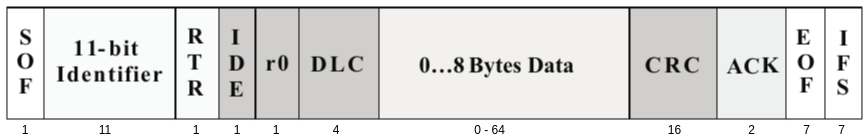
\includegraphics[width=0.8\textwidth]{img/CAN_frame_standard.png}
    \caption{Se muestran los campos de una trama CAN estándar. Debajo de cada campo se indica la cantidad de bits. La imagen se extrajo de \cite{texasSLOA101B}.}
    \label{fig:CAN_frame_standard}
\end{figure}


\begin{figure}[H]
    \centering
    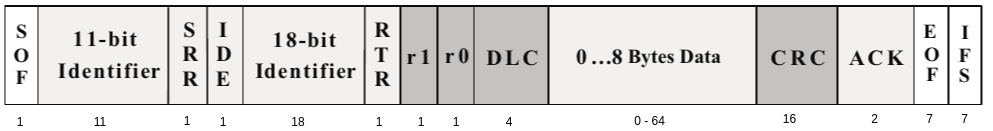
\includegraphics[width=0.8\textwidth]{img/CAN_frame_extended.png}
    \caption{Se muestran los campos de una trama CAN extendida. Debajo de cada campo se indica la cantidad de bits. La imagen se extrajo de \cite{texasSLOA101B}.}
    \label{fig:CAN_frame_extended}
\end{figure}

En el eventual caso en que más de un nodo detecte el medio sin uso, estos querrán transmitir a través del bus. Esta situación se encuentra contemplada por el protocolo y se implementa un mecanismo que resuelve la colisión asegurando la transmisión del mensaje con la prioridad más baja. El primer bit es el campo SOF, seguido del identificador. En la figura \ref{fig:CAN_arbitration} se muestra un ejemplo de este escenario. Tanto el nodo 1 como el nodo 2 quieren utilizar el bus CAN. Ambos comienzan a inyectar su ID correspondiente. En algún momento, ocurre una discrepancia entre el ID inyectado por ambos nodos. Aquel con el campo dominant, es decir 0, gana y completa su transmisión, en este caso el nodo 2. El nodo 1 que quiso envar un 1 por su lado, detecta un 0. Esto genera que detenga su transmisión, dejando que los demás nodos utilicen el medio.

\begin{figure}[H]
    \centering
    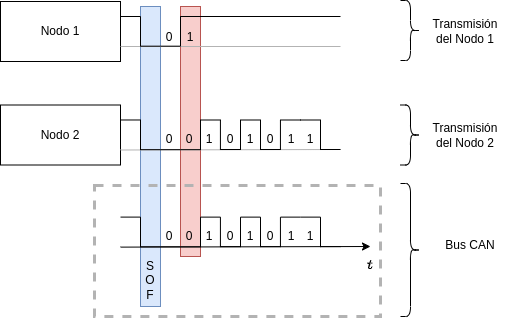
\includegraphics[width=0.6\textwidth]{img/CAN_arbitration.png}
    \caption{Mecanismo para la detección de colisiones. El nodo 2 gana por prioridad y completa su transmisión, mientras que el nodo 1 deja de usar el bus, aguardando a que el nodo 2 finalice.}
    \label{fig:CAN_arbitration}
\end{figure}

En las figuras \ref{fig:CAN_frame_standard} y \ref{fig:CAN_frame_extended} se puede ver que las tramas tienen un campo CRC, el cual es utilizado para que el receptor pueda verificar la integridad del mensaje. Además, se muestra otro campo, el ACK. Cada vez que un nodo recibe un mensaje correctamente, este sobreescribe el bit de ACK con un dominant, es decir un 0.\\

El protocolo CAN base no tiene un acceso al medio controlado por el tiempo, sino que es dominado por eventos (\textit{event-triggered}), ya que varios nodos pueden querer transmitir varios mensajes a la vez, de manera consecutiva. En el estándar ISO 11898-4\cite{ISO11898_4} se define una extensión denominada \textit{Time-Triggered CAN} (TTCAN). A través de una capa de sesión, puede implementarse un acceso al medio dominado por el tiempo.\\

Como se mencionó al principio de la sección \ref{sec:requerimentos_sistema_tolerancia_fallas}, la arquitectura para la tolerancia a fallas no está definida. La elección del protocolo CAN le da versatilidad al uso del bus, ya que puede utilizarse con un acceso al medio tanto controlado por el tiempo como por eventos.